\documentclass[../src/handouts/main.tex]{subfiles}
% note that the CWD (.) above is the output directory of pdflatex
% (<repo-root-dir>/build)

% path that contains required images
\graphicspath{ {../src/handouts/figures/} }

% This document depends on fundamental-concepts.tex, which provides
% the following references (in the order of references in this section):
%   subsec:con-graph-isomorphism
%   thm:con-bipartite-odd-cycle
% As a result, compiling only this document gives undefined references.

% prevent \recall theorems outside this section
% if this section is compiled solely
\def\sectionprefix{intro}%

\begin{document}

\section{Introduction and Mathematical Background}

This section is meant to provide useful background for learning graph theory.

\subsection{Sets}

\begin{definition}{}{intro-set-def}
  (A.1. Definition in text)
  The objects in a set are its \textbf{elements} or \textbf{members}.
  When $x$ is an element of $A$, we write $x \in A$ and say "$x$ \textbf{belongs to} $A$".
  When $x$ is not in $A$, we write $x \notin A$.
  If every element of a set $B$ belongs to $A$, then $B$ is a \textbf{subset} of $A$, and $A$ \textbf{contains} B; we write $B \subseteq A$ or $A \supseteq B$.
\end{definition}

\begin{definition}{}{intro-set-equal}
  (A.3. Definition in text)

  Sets $A$ and $B$ are \textbf{equal}, written $A = B$, if they have the same elements.

  The \textbf{empty set}, written $\emptyset$ or $\lbrace\ \rbrace$ (but not 0), is the unique set with no elements.

  A \textbf{proper subset} of a set $A$ is a subset that is not $A$ itself.
\end{definition}

In \cref{def:intro-set-equal}, notice that there is a special case, in ordered sets, if the orders of the sets $A$ are $B$ not identical, they are not equal. However, in unordered sets, it doesn't matter.

As a result, you need to compare the numbers, elements and orders (in ordered sets) to make sure the two sets are equal.

As for the equal sign, $\equiv$ means logical identity. It differs from $=$.

In \cref{def:intro-set-equal}, we say that zero (0) is not an empty set ($\emptyset$), but in formal proofs, especially in graphs, we need to consider all possible cases, including zero edges, zero vertices. Otherwise, the proofs are only examples.

A subset of a set $A$ \textbf{can} be $A$ itself and an empty set. A proper subset of a set $A$ \textbf{cannot} be $A$ itself, but \textbf{can} be an empty set. (This is likely in the exams.)

\supp{In other words, all subsets of a set $A$ \textbf{include} $A$ itself and an empty set. All proper subsets of a set $A$ \textbf{don't include} $A$ itself, but \textbf{include} an empty set.}

\begin{remark}{Equality of sets}{intro-equal-sets}
  (A.4. Remark in text)
  To prove that $A = B$, we prove that every element of $A$ is in $B$ and that every element of $B$ is in $A$; in other words, $A \subseteq B$ and $B \subseteq A$. It also suffices to turn the description of one set into the description of the other by operations that do not change membership.

  This book proves many characterization theorems for classes of graphs. Such a theorem states that two sets are the same (e.g., the set of bipartite graphs is equal to the set of graphs without odd cycles; \cref{thm:con-bipartite-odd-cycle}).
\end{remark}

As \cref{rem:intro-equal-sets} states, to prove $A = B$, you need to prove both $A \subseteq B$ and $B \subseteq A$ like you do in proving "if and only if" (iff, $\iff$). With only one of the two sides, the answer will be scored half or less.

If you have more than two equal statements, like in Linear Algebra you have 8 equal characteristics, you can use circular proofs. But in Linear Algebra it proves it by two circles with one equality between.

In \cref{rem:intro-equal-sets}, in short, a bipartite graph is a graph with two disjoint and independent sets. An odd cycle is an odd-length cycle.

\begin{remark}{Specifying a set}{intro-specifying-set}
  (A.5 Remark in text)
  Given a set $A$, we may want to specify a subset $S$ consisting of the elements of $A$ that satisfy a given condition. To do so, we write "$S = \{ x \in A:\ \text{condition}(x)\}$". We read this as "$S$ is the set of elements $x$ in $A$ such that $x$ satisfies 'condition' ". For example, the expression $\{ n \in \N : n^2 \leq 25 \}$ is another way to name the set $\{ 1,\, 2,\, 3,\, 4,\, 5 \}$.
\end{remark}

\begin{definition}{}{intro-set-shorthand}
  (A.6. Definition in text)
  When $a,\, b \in \Z$, we write $\{a,\, \ldots,\, b\}$ to represent $\{ i \in \Z: a \leq i \leq b \}$.

  When $n \in \N$, we write $[n]$ for $\{1,\, \ldots,\, n\}$; also $[0] = \emptyset$.

  The set of \textbf{even numbers} is $\{ 2 k : k \in \Z \}$.

  The set of \textbf{old numbers} is $\{ 2 k + 1 : k \in \Z \}$.

  The \textbf{parity} of an integer states whether it is even or odd.
\end{definition}

In \cref{def:intro-set-shorthand}, $[n]$ is similar to $\mathbb{I}_n$ in some other textbooks. Note that the brackets in $[n]$ are not operators like ceiling or flooring. $[0]$ doesn't mean 0, and 0 doesn't mean $\emptyset$.

\begin{definition}{}{intro-partition}
  (A.7. Definition in text)
  A \textbf{partition} of a set $A$ is a list $\clistj{A}{k}$ of subsets of $A$ such that each element of $A$ appears in exactly one subset in the list. (no overlapping)
\end{definition}

Continuing from \cref{def:intro-partition}, in a partition of $A$ into $\clistj{A}{k}$, the sets $\clistj{A}{k}$ in the list can be in one of the following names. They are all the same (except for \textbf{sets}) but used in different scenarios or generations.
\begin{enumerate}
  \item \textbf{Blocks} (In combinatorics; blocks has another definition in the graph theory, so this book prevents using this name.)
  \item \textbf{Classes}
  \item \textbf{Partite sets} (This is only for the sets in a partition of the vertex set of a graph into independent sets.)
  \item \textbf{Independent sets}
  \item \textbf{Sets} (It is not precise enough.)
\end{enumerate}

\begin{remark}{Conventions about universes}{intro-convensions-universes}
  (A.8. Remark in text)
  (Omitted content)
  When we say only that a number is positive without specifying the number system containing it, we mean that it is a positive real number. Thus, "consider $x > 0$" means "let $x$ be a positive real number", but in "for $n \geq 2$, let $G$ be an $n$-vertex graph" our convention is that $n \in \N$.
\end{remark}

In \cref{rem:intro-convensions-universes}, $\N$ is a set of nonnegative integers.
In graph, we usually speak of $n$ as the number of vertices, by context we know that $n$ is a natural number ($n \in \N$ in this text). In the other fields, $n$ may be complex numbers or all integers.

\begin{definition}{}{intro-correspondence}
  (A.9. Definition in text)
  A set $A$ is \textbf{finite} if there is a one-to-one correspondence between $A$ and $[n]$ for some $n \in \N \cup \{0\}$. This $n$ is the \textbf{size} of $A$, written $\abs{A}$.
\end{definition}

In \cref{def:intro-correspondence}, note that 0 is not a set, but $\{ 0 \}$ is a set.

"One-to-one" is ambiguous. it will be covered later in \cref{subsec:intro-function} (\cpagerefrange{subsec:intro-function}{subsec:intro-function-end}), but in brief:
\begin{enumerate}
  \item \textbf{One-to-one correspondence} is a \textbf{bijective function}, means the mapping between two sets \textbf{must cover} all points.
  \item \textbf{One-to-one function} is an \textbf{injective function}, which means the mapping between two sets \textbf{may not cover} all points.
\end{enumerate}

\begin{definition}{}{intro-set-operations}
  (A.11. Definition in text)
  Let $A$ and $B$ be sets.

  Their \textbf{union} $A \cup B$ consists of all elements in $A$ or in $B$ (or both). That's the yellow and green area in ths following figure.

  Their \textbf{intersection} $A \cap B$ consists of all elements in both $A$ and $B$ (green area).

  Their \textbf{difference} $A - B$ consists of the elements of $A$ that are not in $B$.

  Their \textbf{symmetric difference} $A \smalltriangleup B$ is the set of elements belonging to exactly one of $A$ or $B$. It's like the XOR operator.

  The sets are \textbf{disjoint} if their intersection is the empty set $\emptyset$.

  If a set $A$ is contained in some universe $U$ under discussion, then the \textbf{complement} $\bar A$ of $A$ is the set of elements of $U$ \textit{not} in $A$.

  \centering
  \begin{tikzpicture}[
      white/.style = {circle, minimum size=4cm, fill=white},
      yellow/.style = {circle, minimum size=4cm, fill=yellow!50!white},
      green/.style = {circle, minimum size=4cm, fill=green!50!white},
      circ/.style = {draw, very thick, circle, minimum size=4cm},
      rect/.style = {draw, very thick, fill=white, rectangle, minimum height=6cm, minimum width=9cm},
      callout/.style = {rectangle, fill=yellow!50!white, anchor=west}
    ]

    % white U
    \node[rect] at (0, 0) {};

    \begin{scope}
      % yellow A - B and B - A
      \node[yellow] at (-1, 0) {}
      node[yellow] at (1, 0) {};
      % call-out
      \node[callout] at (5, 0) {$\begin{aligned} & A \smalltriangleup B \\ &= (A - B) \cap (B - A) \end{aligned}$};
      % green A and B
      \clip (-1, 0) circle (2);
      \node[green] at (1, 0){};
    \end{scope}

    \node[circ](A) at (-1, 0) {}
    node[circ](B) at (1, 0) {};

    \node at (-5, 0) {\textbf{U}}
    node at (-1, 1.5) {\textbf{A}}
    node at (1, 1.5) {\textbf{B}}
    node at (0, 0) {$A \cap B$}
    node at (-2, 0) {$\stackbelow{A - B}{A \cap \bar B}$}
    node at (2, 0) {$\stackbelow{B - A}{B \cap \bar A}$}
    node at (0, -2.5) {$\left( A \cup B \right)^c = \bar {\left( A \cup B \right)}$};
  \end{tikzpicture}
\end{definition}

\begin{remark}{}{intro-set-element-number}
  (A.13. Remark in text)
  When $A$ and $B$ are sets, $A \smalltriangleup B = (A \cup B) - (A \cap B)$. The union starts with all elements in at least one of $A$ and $B$; we delete those in both.

  When $A$ and $B$ are finite sets, $\abs{A \cup B} + \abs{A \cap B} = \abs{A} + \abs{B}$. Each element of the intersection is counted twice on both sides, each element of the symmetric difference is counted once on both sides, and no other elements are counted.
\end{remark}

\begin{remark}{}{intro-tuple-ordered-pair}
  (A.14. Definition in text)
  A list with entries in $A$ consists of elements of $A$ in a specified order, with repetition allowed. A \textbf{$k$-tuple} is a list with $k$ entries. We write $A^k$ for the set of $k$-tuples with entries in $A$. When $A=\{0,1\}, A^k$ is the set of \textbf{binary $k$-tuples}.

  An \textbf{ordered pair} $(x, y)$ is a list with two entries. The \textbf{cartesian product} of sets $S$ and $T$, written $S \times T$, is the set $\{(x, y): x \in S, y \in T\}$.

  Note that $A^2 = A \times A$ and $A^k = \left\{\left(x_1, \ldots, x_k\right): x_i \in A\right\}$. We read " $x_i$ " as " $x$ sub $i^{\prime}$. When $S = T = \Z$, the cartesian product $S \times T$ is the \textbf{integer lattice} (such a cartesian project covers all integer points on cartesian coordinates, like grids), the set of points in the plane with \textbf{integer coordinates}.
\end{remark}

For the k-tuple in \cref{rem:intro-tuple-ordered-pair}, for example, if $A = \{0, 1\}$ and $k = 2$, the cartesian product $A^2$ is $\{ (0,\, 0),\, (0,\, 1),\, (1,\, 0),\, (1,\, 1) \}$, where all entries are ordered pairs. For $k = 3$, there will be three numbers in each entry. Since $(0,\, 1)$ differs from $(1,\, 0)$, we call it ordered pairs.

\subsection{Quantifiers and Proofs}

In this part, we have no automatic tools, but our hands to write proofs.

Roughly speaking, a mathematical statement is a statement that can be determined to be true or false.
This requires correct mathematical grammar, and it requires that variables be "quantified".

Precisely speaking, they are respectively called \textbf{proposition} and \textbf{predicate}, where predicate is so-called first-order logic.

"It's raining" is a \textbf{proposition}, for we can say this statement is true or false.

The question "do you know my phone number" is not a proposition, but the answer (yes/no) to this question is a proposition.

"Go out" is a imperative, rather than a proposition.

A \textbf{predicate} is "\textbf{for all} $x$ in $S$, the sentence $P(x)$ is true" (for all students in this class, I know their phone number) or "\textbf{for some} $x$ in $S$, the sentence $P(x)$ is true". With a specific range (for all, for some, existing, some, etc.), if we can say it is true or false, this is a predicate.

\begin{definition}{}{intro-quantifiers}
  (A.15. Definition in text)
  In the statement "For all $x$ in $S$, $P(x)$ is true", the variable $x$ is \textbf{universally quantified}. We write this as $(\forall x \in S) P(x)$ and say that $\forall$ is a \textbf{universal quantifier}.

  In "For some $x$ in $S$, $P(x)$ is true", the variable $x$ is \textbf{existentially quantified}. We write this as $(\exists x \in S) P(x)$ and say that $\exists$ is an \textbf{existential quantifier}. The set of allowed values for a variable is its \textbf{universe}.

  Note that in the following table, "helpers" may be absent.

  \centering
  \begin{tabular}{ll|ll}
    Universal ($\forall$) & (Helpers) & Existential ($\exists$) & (Helpers) \\ \hline
    for [all], for every  &           & for some                &           \\
    if                    & then      & there exists            & such that \\
    whenever, for, given  &           & at least one            & for which \\
    every, any            & satisfies & some                    & satisfies \\
    a, arbitrary          & must, is  & has a                   & such that \\
    let                   & be        &                         &
  \end{tabular}
\end{definition}

In the table in \cref{def:intro-quantifiers}, "a graph $\ldots$" and "an integer $\ldots$" without specification of ranges, it means "for all" and is a universal specifier. However, "has a graph $\ldots$" that comes with specification refers to "some" graphs, so "has a" is an existential specifier.

\begin{remark}{}{intro-quantifier-order}
  (A.17. Remark in text)
  The meaning of a statement with more than one quantifier depends on their \textbf{order}. Compare these two sentences:

  (1) "For every graph $G$, there exists $m \in \mathbb{N}$ such that every $v \in V(G)$ has degree at most $m$."

  (2) "There exists $m \in \mathbb{N}$ such that for every graph $G$, every $v \in V(G)$ has degree at most $m$."

  The first statement is \textbf{true}; the second is \textbf{false}.
  Every (finite) graph has a maximum degree, but there is no maximum over all graphs.
  We write the two sentences in logical notation as
  $$
    \begin{aligned}
      (\forall G)(\exists m \in \mathbb{N})(\forall v \in V(G))\left(d_G(v) \leq m\right) \\
      (\exists m \in \mathbb{N})(\forall G)(\forall v \in V(G))\left(d_G(v) \leq m\right)
    \end{aligned}
  $$
\end{remark}

\begin{remark}{Negation of quantified statements}{intro-negation}
  (A.18. Remark in text)
  The logical symbol for negation is $\neg$. If it is false that all $x \in S$ make $P(x)$ true, then there must be some $x \in S$ such that $P(x)$ is false. Similarly, negating an existentially quantified statement yields a universally quantified negation. In notation,

  $$
    \begin{aligned}
      \neg[(\forall x \in S) P(x)] \text{ has the same meaning as } (\exists x \in S)(\neg P(x)). \\
      \neg[(\exists x \in S) P(x)] \text{ has the same meaning as } (\forall x \in S)(\neg P(x)).
    \end{aligned}
  $$

  The universe of quantification does not change when the statement is negated.
  For example, the false statement in \cref{rem:intro-quantifier-order} was

  $$
    (\exists m \in \mathbb{N})(\forall G)(\forall v \in V(G))\left(d_G(v) \leq m\right) .
  $$

  Its negation (which is still false) is the same as

  $$
    (\forall m \in \mathbb{N})(\exists G)\left[\neg\left((\forall v \in V(G))\left(d_G(v) \leq m\right)\right)\right]
  $$
\end{remark}

\begin{definition}{Logical connectives}{intro-logical-connectives}
  (A.19. Definition in text)
  In the following table, we define the operations named in the first column by the truth values specified in the last column.

  \centering
  \begin{tabular}{l|lll}
    Name          & Symbol         & Meaning                & Condition for truth        \\ \hline
    Negation      & $\neg P$       & not $P$                & $P$ false                  \\
    Conjunction   & $P \wedge Q$   & $P$ and $Q$            & both true                  \\
    Disjunction   & $P \vee Q$     & $P$ or $Q$             & at least one true          \\
    Biconditional & $P \iff Q$     & $P$ if and only if $Q$ & same truth value           \\
    Conditional   & $P \implies Q$ & $P$ implies $Q$        & $Q$ true whenever $P$ true
  \end{tabular}
\end{definition}

In "conditional operator $P \implies Q$", if we cannot make $P$ true ($P$ is impossible), $P \implies Q$ is still true, and $P \implies Q$ is meaningless. It is like "if we cannot find an evidence to convict you, you are acquitted". It is a vacuous truth, or vacuous pass in computer-aided design (CAD) coming from no requests to make the condition $P$ existing. For example, $P \implies Q$, in which:
\begin{enumerate*}
  \item $P$ refers to "if TA always tells the truth";
  \item $Q$ refers to "then TA said that this classroom has a hidden treasure can be truth".
\end{enumerate*}
If $P$ is not satisfied; that is, TA does not always tell the truth, then we cannot conclude whether the treasure exists in the classroom or not.

\begin{definition}{}{intro-logical-implication}
  (A.21. Definition in text) In the conditional statement $P \implies Q$, we call $P$ the \textbf{hypothesis} (precondition, premise) and $Q$ the \textbf{conclusion}. The statement $Q \implies P$ is the \textbf{converse} of $P \implies Q$. $P \implies Q$ is $(\neg P) \lor Q$

  Below we list ways to say $P \implies Q$ in English. (The instructor won't ask you to fill in the blanks in the last two statements given $P \implies Q$ in the exams.)
  \begin{enumerate}
    \item If $P$ (is true), then $Q$ (is true).
    \item $Q$ is true whenever $P$ is true.
    \item $Q$ is true if $P$ is true.
    \item $P$ is true only if $Q$ is true.
    \item \textbf{$P$ is a sufficient condition for $Q$.} (You need to ensure $P$ true before checking $Q$ true, so $P$ true is the prerequisite.)
    \item \textbf{$Q$ is a necessary condition for $P$.} (Given $P$ true, $Q$ is the deterministic factor to make $P \implies Q$ true or false.)
  \end{enumerate}
\end{definition}

\subsubsection{More Examples of Predicate Logic}

Express "Andy and Paul have the same biological maternal grandmother" in logic.
\begin{enumerate}
  \item Let $M(x, y)$ denote that $x$ is $y$'s mother. Consider
    $$
      \forall x \forall y \forall u \forall v(M(x, y) \land M(y, \text{Andy}) \land M(u, v) \land M(v, \text{Paul}) \implies x = u)
    $$
    Do you find out something weird?
    \begin{enumerate}
      \item First, not all $x,\, y,\, u,\, v$ satisfy the logical expression above.
      \item Secondly, without specifying $x$ and $u$ in the precondition, you cannot make $x$ and $y$ identical.
      \item Lastly, $y,\, \text{Andy},\, v,\, \text{Paul}$ have many mothers in the logical expression.
    \end{enumerate}
  \item Let $m(x)$ denote $x$'s biological mother. The following logical expression matches the English version.
    $$
      m(m(\text{Andy}))=m(m(\text{Paul})).
    $$
    Since everyone has exactly one biological mother, we introduce a function $m(x)$ to denote this fact. This is a unction to capture a single object.
\end{enumerate}

\subsubsection{Direct, Contrapositive and Contradiction Method}

\begin{remark}{Providing implications}{intro-proving-methods}
  (A.23. Remark in text)
  The \textbf{direct method} of proving $P \implies Q$ is to assume that $P$ is true and then to apply mathematical reasoning to deduce that $Q$ is true.
  When $P$ is "$x \in A$" and $Q$ is $Q(x)$, the direct method considers an \textit{arbitrary} $x \in A$ and deduces $Q(x)$.
  There is no "proof by example".
  The proof must apply to every member of $A$ as a possible instance of $x$.

  The \textbf{contrapositive} of $P \implies Q$ is $\neg Q \implies \neg P$. Each of these statements fails only when $P$ is true and $Q$ is false. Thus, they are equivalent; we can prove $P \implies Q$ by proving $\neg Q \implies \neg P$. This is \textbf{contrapositive method}.

  We have observed that $(P \implies Q) \iff \neg \left[ P \land (\neg Q) \right]$.
  Hence, we can prove $P \implies Q$ by proving that $P$ and $\neg Q$ cannot both be true.
  We do this by obtaining a contradiction after assuming both $P$ and $\neg Q$.
  This is the \textbf{method of contradiction}.
\end{remark}

There are some notes for \cref{rem:intro-proving-methods}:
\begin{enumerate}
  \item Contrapositive method means the same logic in the other words instead of reversing the words.
  \item Although $Q \implies P$ is the \textbf{converse} (like reverse) of $P \implies Q$, the two statements have different meanings, and a \textbf{converse} of $A$ is not a \textbf{contrapositive} of $A$.
  \item Contrapositive method and contradiction method are indirect proofs.
  \item The method of \textbf{contradiction} is not the \textbf{contrapositive} method.
  \item All the three methods work, but you may want to pick a method that you're familiar with and is the shortest proof you need to write. Learn proving methods/techniques as many as possible if you don't know which method is the most appropriate. And ensure the order of proving right beforehand. These tools are useful in writing a thesis because solving a reduced and equivalent problem may be more easy than solving the original problem directly.
\end{enumerate}

\begin{remark}{Biconditional statements}{intro-biconditional}
  (A.24. Remark in text)
  The biconditional statement "P \iff Q" has the same meaning as "$(P \implies Q) \land (Q \implies P)$". We read it as "$P$ if and only if $Q$", where "$P \implies Q$ is "$P$ if $Q$", and "$P \implies Q$" is "$P$ only if $Q$".
\end{remark}

\subsection{Lemma, Theorem, Proposition and Corollary}

The explanations of these four words:
\begin{enumerate}
  \item \textbf{Lemma}: It's a premise. It is a lesser statement, and is usually proven to help prove the other statements.
  \item \textbf{Theorem}: It's a thesis to be proven. Thus, theorem is a major result requiring some efforts.
  \item \textbf{Proposition}: It's something proposed to be proven (true or false), and typically it takes less effort than a theorem.
  \item \textbf{Corollary}: It means \textit{gift} in Latin, and it follows easily from a theorem or proposition without much additional work. Corollary is a sub-theorem.
\end{enumerate}

Although these words come before some graphs or paragraphs, it doesn't mean that you need to memorize them, but they are commonly used or crucial in the later paragraphs or subsections.

You shouldn't read a corollary before reading its prerequisite lemma/theorem/proposition.

\subsection{Induction and Recurrence}

\begin{principle}{Well-ordering principle (property)}{intro-wop}
  For the natural numbers: every non-empty subset of $N$ has a least (smallest) element.
  This is an \textbf{axiom}, as parts of our intuitive understanding of what $N$ is.
\end{principle}

\begin{principle}{Principle of induction (Mathematical induction)}{intro-induction}
  (A.25. Theorem in text)
  For each natural number $n$, let $P(n)$ be a mathematical statement.
  If properties (1) and (2) below hold, then for each $n \in \N$ the statement $P(n)$ is true.
  \begin{enumerate}
    \item Base case: P(1) is true.
    \item Induction: For $k \in \N$, $P(k)$ is true, then $P(k + 1)$ is true.
  \end{enumerate}
\end{principle}

\textbf{Proof} of \cref{princ:intro-induction}:
If $P(n)$ is not true for all $n \in \N$, then the set of natural numbers where it fails is nonempty.
By the \textbf{well ordering property}, there is a least (smallest) natural number in this set.
By (1), this number cannot be 1.
By (2), it cannot be bigger than 1.
The contradiction implies that $P(n)$ is true for all $n \in \N$.

Notes for \cref{princ:intro-induction}:
\begin{enumerate}
  \item The principle of induction relies on the well ordering property of integers. If the base case (basis case or assumption) is wrong, the induction is totally wrong. You should prove the basis before the induction step. Otherwise, garbage in, garbage out.
  \item The base case is not always 1.
  \item It's not always to prove $P(\bm{k + 1})$ true under $P(k)$ true. It's possible for you to prove $P(k)$ true under $P(\bm{k - 1})$ true for the ease of proofs; such a case still follows the well-ordering principle which proves the principle of induction.
  \item Mathematical induction has many variances. $n$ may be in the set of even numbers, or the set of odd numbers; $n$ may be even zero. It all depends on the domain of $n$. In different cases, the base case can differ.
  \item In section 1.3, we will talk about induction template and induction trap (pitfall). \supp{For the induction trap, in brief, since we don't prove $P(k)$ true ($P(k)$ true is a hypothesis to prove $P(k + 1)$ true), $P(k + 1)$ may be true under an impossible assumption "$P(k)$ true". In section 1.3, you may find a certain upperbound for $n$, so you need to use another technique.} % TODO: link to section 1.3.
\end{enumerate}

\begin{proposition}{}{intro-line-region}
  (A.26. Proposition in text)
  If $S$ is a set of $n$ lines in the plane such that every two have exactly one common point and no three have a common point, then $S$ cuts the plane into $\left[ 1 + \frac{n (n + 1)}{2} \right]$ regions.
\end{proposition}

\textbf{Proof} of \cref{prop:intro-line-region}:

We use induction on $n$ to prove the claim for all $n \in \N$.
Let $P(n)$ be the statement that the claim holds for all such sets of $n$ lines.

Basis step ($P(1)$): With one line the number of regions is 2, which equals $\left[ 1 + \frac{1 (n + 1)}{2} \right]$.

Induction step ($P(k) \implies P(k + 1)$): The statement $P(k)$ is the induction hypothesis. Let $S$ be a set of $k + 1$ lines meeting the conditions. Select a line $L$ in $S$, where the line is the dashed line in \cref{fig:intro-line-region-additional}, and let $S'$ be the set of $k$ lines obtained by deleting $L$ from $S$.

\begin{figure}[ht]
  \centering
  \begin{tikzpicture}[]
    \draw (0, 3) -- (3, 0);
    \draw (0, 2) -- (3, 2);
    \draw[dashed] (0, 0) -- (3, 3);
  \end{tikzpicture}
  \caption{An additional line (dashed one) for the demonstration of \cref{prop:intro-line-region}.}
  \label{fig:intro-line-region-additional}
\end{figure}

Since $S'$ meets the conditions, the induction hypothesis states that $S'$ cuts the plane into $1 + \frac{k (k + 1)}{2}$ regions.
When we replace $L$, some regions are cut.
The increase in the number is the number of regions that $L$ cuts. It moves from one of these regions to another each time it crosses a line in $S'$.
Since $L$ crosses each line in $S'$ once, then line in $S'$ cut $L$ into $\bm{k + 1}$ \textbf{pieces}. (It is a lemma that a line cuts a region into two)
Each piece corresponds to a region that $L$ cuts.

Thus, the number of regions formed by $S$ is $k + 1$ more than the number of regions formed by $S'$.
The number of regions formed by $S$ is
$$
  1 + \frac{k (k + 1)}{2} + \bm{(k + 1)} = 1 + \frac{(k + 1)((k + 1) + 1)}{2}.
$$
We have proved that $P(k)$ implies $P(k + 1)$.

By the principle of induction, the claim holds for every $n \in \N$.

\supp{In this proof, it shows the case of $k + 1$ before $k$, and proves from $k$ to $k + 1$. This is common in text.}

\subsubsection{Example A.29}

Recurrent means for a given function $f$, $f(n)$ depends on some of previous results $f(n - 1),\, f(n - 2),\, \ldots$. In spanning trees and graph coloring problems, recurrence is used.
% TODO: link to spanning trees and graph coloring problems

Let $a_1,\, a_2,\, \ldots$ be defined as follows. And our goal is to seek for a formula for $a_n$ in terms of $n$.
$$
  \begin{cases}
    a_1 & = 2                                                   \\
    a_2 & = 8                                                   \\
    a_n & = 4 (a_{n - 1} - a_{n - 2}) \ \ \text{for}\, n \geq 3
  \end{cases}
$$

We may try to guess a formula that fits the data.
The definition yields the following three values as follows.

$$
  \begin{cases}
    a_3 & = 24  \\
    a_4 & = 64  \\
    a_5 & = 160
  \end{cases}
$$

All of them satisfy $a_n = n 2^n$.
Having guessed this as a possible formula for $a_n$, we can try to use induction to prove it.

When $n = 1$, we have $a_1 = 2 = 1 \cdot 2^1$.
When $n = 2$, we have $a_2 = 8 = 2 \cdot 2^2$.
In both cases, the formula is correct.

In the induction step, we prove that the desired formula is correct for $n \geq 3$.
We use the hypothesis that the formula is correct for the preceding instances $n - 1$ and $n - 2$.
This allows us to compute $a_n$ using its expression in terms of earlier value:

$$
  \begin{aligned}
    a_n & = 4 (a_{n - 1} - a_{n - 2})                             \\
        & = 4 \left[ (n - 1) 2^{n - 1} - (n - 2) 2^{n -2} \right] \\
        & = (2 n - 2) 2^n - (n - 2) 2^n                           \\
        & = n 2^n                                                 \\
  \end{aligned}
$$

The validity of the formula for $a_n$ allows from its validity for $a_{n -1}$ and $a_{n - 2}$, which completes the proof.

\subsection{Functions}\label{subsec:intro-function}

\begin{definition}{}{intro-function}
  (A.30. Definition in text)
  A \textbf{function} $f$ from a set $A$ to a set $B$ assigns to each $a \in A$ a single element $f(a)$ in $B$, called the \textbf{image} of $a$ under $f$.
  For a function $f$ from $A$ to $B$ (written \defaultfunc), the set $A$ is the \textbf{domain} and the set $B$ is the \textbf{target} (\textbf{codomain}). The \textbf{image} of a function $f$ with domain $A$ is $\{ f(a):\, a \in A \},$.
\end{definition}

In brief, a \textbf{function} transforms (maps) elements of one set into elements of another set.

Examples of functions: absolute value function, polynomial function like $x^2 + 1$, \textit{size} of a set, etc. \textit{size} is a function whose domain is the set of finite sets and whose target is $\N \cup \{0\}$.

\begin{definition}{}{intro-floor-ceil-sequence}
  (A.31. Definition ins text)
  For $x \in \R$, the \textbf{floor} $\floor{x}$ is the greatest integer that is at most $x$.
  The \textbf{ceiling} $\ceil{x}$ is the smallest integer that is at least $x$.
  A \textbf{sequence} is a function $f$ whose domain is $\N$.
  A \textbf{sequence} is "$a_1,\, a_2,\, a_3,\, \ldots$", where $a_i = f(i)$.
\end{definition}

For the floor and ceiling functions, you could check \cref{table:intro-ex-floor-ceil} for some examples.

\begin{table}[ht]
  \def \gap {\\[-0.5em]}
  \centering
  \begin{tabular}{ccc}
    \hline \gap
    $x$  & Floor $\floor{x}$ & Ceiling $\ceil{x}$ \gap \\ \hline
    2.4  & 2                 & 3                       \\
    2    & 2                 & 2                       \\
    -2.7 & -3                & -2                      \\ \hline
  \end{tabular}
  \caption{Examples of floor and ceiling functions}
  \label{table:intro-ex-floor-ceil}
\end{table}

\begin{remark}{Schematic representation}{intro-repr}
  (A.32. Remark in text)
  A function \defaultfunc is \textbf{defined on} A and \textbf{maps} A into B.
  To visualize a function \defaultfunc, we draw a region representing $A$ and a region representing B, and from each $x \in A$ we draw an arrow to $f(x)$ in $B$.
  In diagraph language, this produces an orientation of bipartite graph with partite sets $A$ and $B$ in which every element of $A$ is the tail of exactly one edge (pair $(a, f(a))$).

  \centering
  %TODO: make the TikZ version
  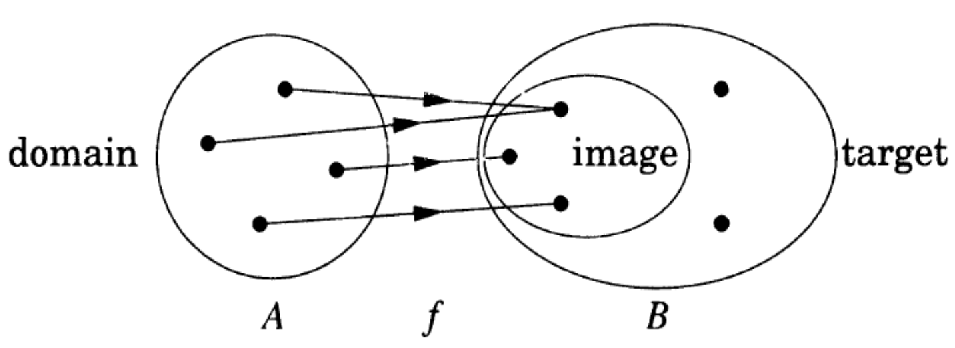
\includegraphics[width=.5\textwidth]{intro-function}
\end{remark}

In \cref{rem:intro-repr}, we can see that \textbf{image} is a subset of \textbf{target}. (See \cref{def:intro-function} for their definition.)

\begin{definition}{}{intro-bijection}
  (A.33. Definition in text)
  A function \defaultfunc is a \textbf{bijection} if for every $b \in B$ there is exactly one $a \in A$ such that $f(a) = b$.
\end{definition}

Relationships between each two of domain, target (codomain) and image can be one of the following three special functions: bijective, surjective and bijective functions.

\begin{reusablefigure}
  \centering
  % TODO: make a TikZ version
  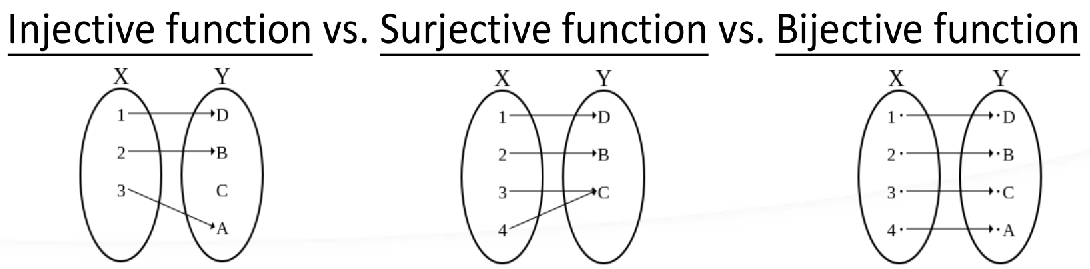
\includegraphics[width=.5\textwidth]{intro-special-functions}
  \caption{Illustration for three special functions: injective, surjective and bijective functions}
  \label{fig:intro-special-functions}
\end{reusablefigure}

\textbf{Injective function} (\textbf{injection (function)}):
\begin{enumerate*}
  \item It means each distinct element in its (such a function's) codomain corresponds to an distinct element in its domain, and vice versa. ($x_1 \neq x_2 \implies f(x_1) \neq f(x_2)$)
  \item It's possible for an injective function to map an element in its codomain to nothing in its domain like the element $C$ in \cref{fig:intro-special-functions}.
  \item Some books call it "one-to-one function", but don't be confused with "one-to-one correspondence" (bijection).
\end{enumerate*}

\textbf{Surjective function} (\textbf{surjection (function)}):
\begin{enumerate*}
  \item It is also known as an \textbf{onto function}. Onto functions are more commonly used.
  \item It means every element $y$ in its codomain can find at least one element $x$ in its domain such that $f(x) = y$. So, some elements in its domain may map to the same element in its codomain like 3 and 4 in \cref{fig:intro-special-functions}.
  \item In other words, its image is equal to its codomain.
\end{enumerate*}

\textbf{Bijective function} (\textbf{bijection (function)}):
\begin{enumerate*}
  \item It is so-called \textbf{one-to-one correspondence}, but don't be confused with the one-to-one function (injection). You could use only bijective function.
  \item Such a function is both injective and surjective.
  \item It means the sizes of the its domain and its codomain are identical, and each element in its domain maps to a distinct element in its codomain.
  \item In \cref{subsec:con-graph-isomorphism}, we may encounter two different-looking graphs with identical structures. To prove two graphs are \textbf{isomorphic}, we utilize the characteristics of the one-to-one correspondence (\textbf{bijective} function) from nodes and edges of a graph to those of the other graph.
\end{enumerate*}
\vspace{1em}

\begin{example}{Pairing spouses}{intro-spouse}
  (A.34. Example in text)
  Let $M$ be the set of men at a party, and let $W$ be the set of women.
  If the attendees consist entirely of married couples, then we can define a function \func{f}{M}{W} by letting $f(x)$ be the spouse of $x$.
  For each woman $w \in W$, there is exactly one $x \in M$ such that $f(x) = w$.
  Hence, $f$ is a bijection from $M$ to $W$.
\end{example}

\begin{definition}{}{intro-inverse}
  (A.35. Definition in text)
  If $f$ is a bijection from $A$ to $B$, then the \textbf{inverse} of $f$ is the function \func{g}{B}{A} such that, for each $b \in B$, $g(b)$ is the unique element $x \in A$ such that $f(x) = b$.
  We write $f^{-1}$ for the function $g$.
\end{definition}

\begin{definition}{}{intro-composition}
  (A.36. Definition in text)
  If we have \defaultfunc and \func{g}{B}{C}, then the \textbf{composition} of $g$ with $f$ is a function \func{h}{A}{C} defined by $h(x) = g(f(x))$ for $x \in A$.
  When $h$ is the composition of $g$ with $f$, we write $h = g \circ f$.

  \centering
  % TODO: TikZ version
  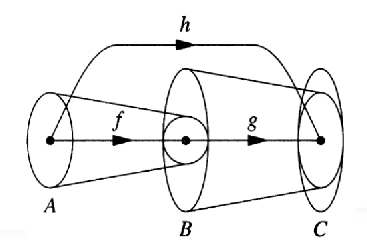
\includegraphics[width=.3\textwidth]{intro-composition}
\end{definition}

\label{subsec:intro-function-end}

\subsection{Counting and Binomial Coefficients (Skipped)}

This part is covered in senior high schools.

"$n$ choose $k$" (A.42 Theorem in text):
\begin{equation}
  \left(\begin{array}{c} n \\ k \end{array}\right) = C^n_k = \frac{n!}{k! (n - k)!}
  \label{eq:intro-combination}
\end{equation}

Pascal's formula/rule (A.48 Lemma in text):
\begin{equation}
  \text{If } n \geq 1 \text{, then } \C{n}{k} = \C{n - 1}{k} + \C{n - 1}{k - 1}
  \label{eq:intro-pascal}
\end{equation}

\subsection{Relations}

Given two objects $s$ and $t$, not necessarily of the same type, we may ask whether they satisfy a given \textbf{relationship}.
Let $S$ denote the set of objects of the first type, and let $T$ denote the set of objects of the second type.
Some of the ordered pairs $(s,\, t)$ may satisfy the \textbf{relationship}, and some may not.
\Cref{def:intro-relation} makes this notion precise.

In brief, a relationship (denoted by $\times$) is between two sets, but no need to be the same type. Functions are relations as well.

\begin{definition}{}{intro-relation}
  (A.50. Definition)
  When $S$ and $T$ are sets, a \textbf{relation} between $S$ and $T$ is a subset of the cartesian product $S \times T$ (\cref{rem:intro-tuple-ordered-pair} in \cpageref{rem:intro-tuple-ordered-pair}).

  A \textbf{relation on} $S$ is a subset of $S \times S$.
\end{definition}

For \cref{def:intro-relation}, in other words, if there is a relation between two sets, such a relationship can be denoted pair by pair (pairwisely).

Note that the subnet of $S \times T$ can be an empty set, one or some of pairs in $S \times T$ and $S \times T$. See \cref{def:intro-set-equal} and its notes in \cpageref{def:intro-set-equal} for more info.

For example, given two sets $D = \{ 1,\, 2\}$ and $C = \{ A,\, B \}$, their possible unordered relations are the cartesian product $D \times C$, which is $(1,\, A),\, (1,\, B),\, (2,\, A),\, (2,\, B)$. If the relations are ordered, there will be $D \times C$ and $C \times D$. Unordered relations are more common. See \cref{rem:intro-tuple-ordered-pair} in \cpageref{rem:intro-tuple-ordered-pair} for more info.

Relations are common for transitions in graphs:
\begin{enumerate*}
  \item A graph $G$ consists of vertices $V(G)$ and edges $E(G)$. For some $v \in V(G)$ and $e \in E(G)$, we have the following two kinds of relations.
  \item \textbf{Incidence relation} is a set of ordered pairs $(v,\, e)$, where vertex $v$ is an endpoint of edge $e$. In brief, it's the relations between each two of vertices and edges.
  \item \textbf{Adjacency relation} is a relation on $V(G)$ containing the set of ordered vertex pairs $(x,\ y)$ such that $x$ and $y$ are the endpoints of some edge(s). In brief, it's the relations between each two vertices.
  \item In \cref{fig:intro-relation}, let $S = \left\{ S_1,\, S_2 \right\}$ denote all possible states. All possible relations (transitions) are $S \times S$, which includes four elements in directed graph like in \cref{fig:intro-relation}, but includes three elements in undirected graph (because $(S_1,\, S_2)$ and $(S_2,\, S_1)$ are the same edge).
  \item If a graph is not a simple graph, there can be multiple edges between some two vertices, and can be multiple loops on some vertices. So, there may be multiple adjacency relation.
\end{enumerate*}

\begin{figure}[ht]
  \centering
  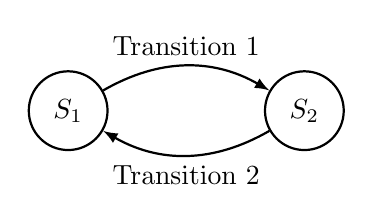
\begin{tikzpicture}[thick,
      main/.style = {draw, circle, minimum size=10mm},
      arrow/.style = {-latex},
      auto]
    % nodes
    \node[main] (1) at (0, 0) {$S_1$};
    \node[main] (2) at (3, 0) {$S_2$};

    % directed edges
    \draw[arrow] (1) to[bend left=30] node[above] {Transition 1} (2);
    \draw[arrow] (2) to[bend left=30] node[below] {Transition 2} (1);
  \end{tikzpicture}
  \caption{Illustration for relations}
  \label{fig:intro-relation}
\end{figure}

\begin{recallable}{definition}{}{intro-equiv-relation}
  (A.52. Definition in text)
  An \textbf{equivalence relation} on a set $S$ is a relation $R$ on $S$ such that for all choices of distinct $x,\, y,\,z \in S$ satisfy the following three properties:
  \begin{enumerate*}
    \item \textbf{Reflexive property}: $(x,\, x) \in R$.
    \item \textbf{Symmetric property}: $(x,\, y) \in R$ implies $(y,\, x) \in R$.
    \item \textbf{Transitive property}: $(x,\, y) \in R$ and $(y,\, z) \in R$ imply $(x,\, z) \in R$.
  \end{enumerate*}
\end{recallable}

An example for \cref{def:intro-equiv-relation} could be the graph isomorphism (denoted by $\triangleq$ or $\cong$ introduced in \cref{subsec:con-graph-isomorphism}), which means graphs are \textit{equal in some sense}. Note that graph isomorphism is related to graph instead of values (number of vertices and edges) or logics (truth table).

A real-life example for \cref{def:intro-equiv-relation} (but not exactly matched) could be as follows. Let $S$ be the set of all people in your family tree, and let $R$ denote all relations in law in the same family tree. You can see an equivalence relation as follows.
\begin{enumerate*}
  \item Reflexive property: You and yourself have relationship.
  \item Symmetric property: You and one of your cousin have relationship in law and vice versa.
  \item Transitive property: "You and your cousin's relationship" and "your cousin and his father's relationship" imply "you and your cousin's father's relationship".
  \item The above-mentioned three properties apply to all choices of people in your family tree.
\end{enumerate*}
In this case, if $R$ denotes all immediate relationships (IR)\footnote{Immediate relationships are direct familial connections such as parents, siblings, children, spouse, grandparents, and grandchildren.}, "you and your father's IR" and "your father and your uncle's IR" don't imply "you and your uncle's IR".

\subsection{Pigeonhole Principle}

Simple statements: If there are $n$ holes and $n + 1$ pigeons, and all pigeons are in the holes, then there must be at least one hole with two pigeons.

Formal statements: \cref{princ:intro-pigeonhole}

\begin{principle}{Pigeonhole Principle}{intro-pigeonhole}
  (A.57. Lemma in text)
  If a set consisting of more than $kn$ objects is partitioned into $n$ classes,then some class receives more than $k$ objects.
\end{principle}

\textbf{Proof} of \cref{princ:intro-pigeonhole}: The contrapositive states that if every class receives at most $k$ objects, then in total there are at more $kn$ objects.

\Cref{princ:intro-pigeonhole} need not be proven later, for it is a lemma.

\subsection{Optimization and Complexity (Skipped)}

\end{document}